\documentclass{article}
\usepackage{iclr2025_conference,times}
\input{math_commands.tex}

\usepackage{hyperref}
\usepackage{url}
\usepackage{graphicx}
\usepackage{booktabs}
\usepackage{amsmath}
\usepackage{xcolor}
\usepackage{multirow}
\usepackage{array}
\usepackage{tabularx}
\usepackage{tikz}
\usepackage{pgfplots}
\pgfplotsset{compat=1.18}
\usetikzlibrary{arrows.meta,positioning,shapes.geometric}

\title{Optimizing GLM-ASR Inference with Custom Triton Kernels:\\Flash Attention, Kernel Fusion, and fp16 Pipelining}

\newcommand{\fix}{\marginpar{FIX}}
\newcommand{\new}{\marginpar{NEW}}
\newcommand{\chg}[1]{{\color{blue}#1}}
\newcommand{\chgcell}[1]{\textcolor{blue}{#1}}
\newcommand{\chglabel}{{\setlength{\fboxsep}{1pt}\colorbox{yellow!45}{\textcolor{red}{\scriptsize CHANGED}}}}
\newcommand{\latestchglabel}{{\setlength{\fboxsep}{1pt}\colorbox{yellow!65}{\textcolor{black}{\scriptsize LATEST CHANGE}}}}
\newcommand{\latestchgblock}[1]{%
  \begingroup
  \setlength{\fboxsep}{4pt}%
  \colorbox{yellow!20}{%
    \parbox{\dimexpr\linewidth-2\fboxsep\relax}{#1}%
  }%
  \endgroup
}
\newcommand{\latestsource}[1]{%
  \par\noindent
  {\footnotesize \latestchglabel\ \parbox[t]{0.9\linewidth}{#1}}\par
}
\newcolumntype{Y}{>{\raggedright\arraybackslash}X}

\begin{document}
\maketitle

% Abstract omitted to maximize main body content within 8-page limit.

%======================================================================
\section{Introduction}\label{sec:motivation}
%======================================================================

\subsection{Motivation}

Current computational demands of transformer-based ASR models and limited inference budgets have driven the need for efficient GPU kernel implementations that can process audio faster than playback speed.
This has instigated the investigation and development of custom kernel optimizations for real-time speech recognition, particularly for latency-constrained applications such as live captioning, voice assistants, and conference transcription.
GLM-ASR is a multimodal encoder--decoder model that converts raw audio waveforms into text through a pipeline of compute-intensive transformer layers.
Its inference workload is dominated by matrix multiplications, attention computations, and element-wise operations---all of which are amenable to GPU acceleration through custom kernels.

GPU kernel optimization matters because default PyTorch operators do not exploit hardware-specific features such as extended shared memory, tensor-core-friendly data layouts, or operation fusion across kernel boundaries.
We design and optimize a complete working implementation using Triton~\citep{tillet2019triton} to create custom GPU kernels.
By writing custom kernels, we can fuse multiple operations into a single kernel launch, tune tile sizes to the GPU's shared memory capacity, and select data types that maximize throughput---eliminating the intermediate video RAM (VRAM) round-trips that dominate latency in the default implementation.

The principal constraint is the kernel design space, as tile dimensions, warp counts, pipeline stages, and data types interact in non-obvious ways, and a configuration that works on one GPU architecture may fail or regress on another.
We validated our parameter choices through a 22-configuration ablation study on the H200 (Section~\ref{sec:optimization}).

\subsection{System Overview}

We determine that our optimal approach is to implement the compute-intensive operations as fused Triton kernels while delegating matrix multiplications to cuBLAS, following the \textbf{Triton track} with all required kernels in \texttt{layers.py}, \texttt{attention.py}, and \texttt{rope.py}.
Table~\ref{tab:kernels} lists the ten kernels implemented, and Figure~\ref{fig:asr-pipeline} illustrates where they operate in the inference pipeline.
We test each component individually and integrate them in a bottom-up fashion, verifying correctness at each stage before proceeding to performance tuning.

\begin{table}[h]
\centering
\caption{Implemented Triton kernels and their roles.}
\label{tab:kernels}
\small
\begin{tabular}{@{}llll@{}}
\toprule
\textbf{Kernel} & \textbf{File} & \textbf{Phase} & \textbf{Purpose} \\
\midrule
\texttt{gelu\_kernel} & layers.py & Encoder MLP & GELU activation \\
\texttt{silu\_kernel} & layers.py & Decoder MLP & SiLU activation \\
\texttt{rmsnorm\_kernel} & layers.py & Decoder norms & RMSNorm + fp16 output \\
\texttt{layernorm\_kernel} & layers.py & Encoder norms & LayerNorm + fp16 output \\
\texttt{linear\_kernel\_tf32} & layers.py & Matmul & General Matrix Multiply (GEMM) \\
\texttt{fused\_swiglu\_kernel} & layers.py & Decoder MLP & Fused SwiGLU \\
\texttt{fused\_linear\_gelu\_kernel} & layers.py & Encoder MLP & Fused Linear+GELU \\
\texttt{flash\_attention\_kernel} & attention.py & Attention & Flash Attention \\
\texttt{fused\_rope\_pair\_kernel} & rope.py & Attention & Fused Q+K RoPE \\
\texttt{compute\_freqs\_kernel} & rope.py & Attention & Frequency precompute \\
\bottomrule
\end{tabular}
\end{table}

\begin{figure}[h]
\centering
\small
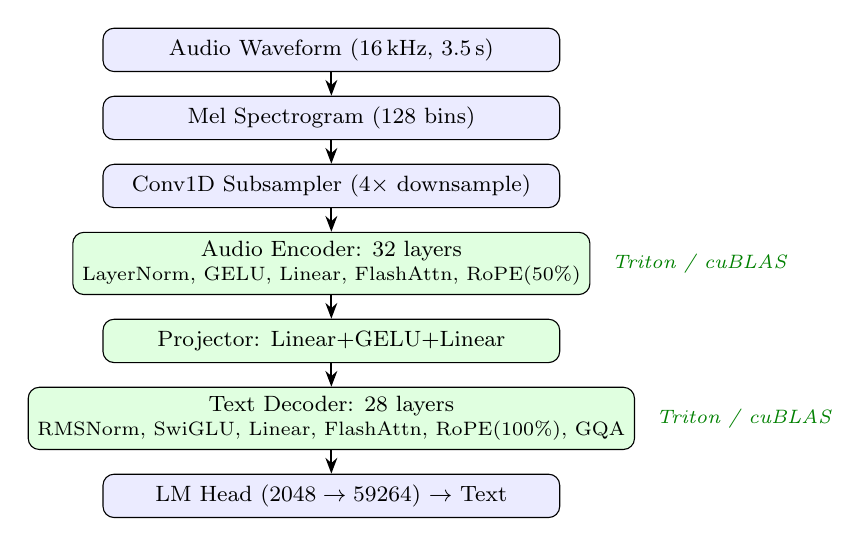
\begin{tikzpicture}[
    node distance=0.3cm,
    block/.style={draw, rounded corners, minimum width=5.8cm, minimum height=0.55cm, font=\footnotesize, align=center, fill=blue!8},
    arrow/.style={-{Stealth[length=2mm]}, thick},
  ]
  \node[block] (audio) {Audio Waveform (16\,kHz, 3.5\,s)};
  \node[block, below=of audio] (mel) {Mel Spectrogram (128 bins)};
  \node[block, below=of mel] (conv) {Conv1D Subsampler ($4\times$ downsample)};
  \node[block, below=of conv, fill=green!12] (enc) {Audio Encoder: 32 layers\\[-1pt] {\scriptsize LayerNorm, GELU, Linear, FlashAttn, RoPE(50\%)}};
  \node[block, below=of enc, fill=green!12] (proj) {Projector: Linear+GELU+Linear};
  \node[block, below=of proj, fill=green!12] (dec) {Text Decoder: 28 layers\\[-1pt] {\scriptsize RMSNorm, SwiGLU, Linear, FlashAttn, RoPE(100\%), GQA}};
  \node[block, below=of dec] (out) {LM Head ($2048 \to 59264$) $\to$ Text};
  \foreach \a/\b in {audio/mel, mel/conv, conv/enc, enc/proj, proj/dec, dec/out}
    \draw[arrow] (\a) -- (\b);
  \node[right=0.15cm of enc, font=\scriptsize\itshape, text=green!50!black] {Triton / cuBLAS};
  \node[right=0.15cm of dec, font=\scriptsize\itshape, text=green!50!black] {Triton / cuBLAS};
\end{tikzpicture}
\vspace{-1ex}
\caption{GLM-ASR pipeline.  Shaded stages use our Triton kernels (or cuBLAS for matmul).}
\label{fig:asr-pipeline}
\end{figure}

In addition to the required kernels, we implement four additional optimizations: (1)~a KV-cached generation loop (\texttt{generate\_v8b}) that reduces decoding from $O(n^2)$ to $O(n)$, (2)~an end-to-end fp16 precision pipeline that halves memory traffic, (3)~a \texttt{GPUProfile} system that adapts tile sizes to the target GPU at import time, and (4)~a PyTorch Scaled Dot-Product Attention (SDPA) fallback for single-token decode steps where kernel launch overhead exceeds computation cost.
Each subcomponent is modular in order to produce a robust, adaptable and portable system.

\textbf{Headline results.}  Upon completion of this project, our final implementation achieves \textbf{204.8\,ms} end-to-end latency on an H200 MIG~3g.71gb partition (baseline: 464.1\,ms), a \textbf{2.27$\times$ speedup} with \textbf{100\% transcription accuracy}.  On an RTX~5090, the same code achieves \textbf{100.4\,ms} (2.61$\times$).


%======================================================================
\section{Implementation}\label{sec:implementation}
%======================================================================

\subsection{Implementation Summary}

The GLM-ASR inference pipeline (Figure~\ref{fig:asr-pipeline}) has five computational phases, each with distinct performance characteristics.
We employ a performance-budgeting technique to attribute latency to each stage and identify where optimization effort would yield the largest gains.

\textbf{Phase~1: Mel Spectrogram + Conv1D Subsampling.}
Converts raw 16\,kHz audio to 128-bin Mel features and downsamples 4$\times$ via strided 1D convolutions.  These are PyTorch built-in operations (read-only \texttt{conv.py}), which we do not modify.  The phase is bandwidth-bound due to large feature maps with simple arithmetic.

\textbf{Phase~2: Audio Encoder (32 layers).}
Each layer applies LayerNorm, self-attention (20 heads, $d_k$=64), and a two-layer multi-layer perceptron (MLP) with GELU activation.  Rotary Position Embedding (RoPE)~\citep{su2024roformer} is applied to 50\% of head dimensions (the first 32 of 64 are rotated, as specified by the model architecture).  On the H200, our flash attention kernel achieves an AI of $\sim$112 for encoder attention (Section~\ref{sec:bottleneck}), well above the GPU's ridge point---the threshold where compute and memory bandwidth are equally limiting.  This makes encoder attention compute-bound (limited by arithmetic throughput) on the H200, but a naive 3-kernel implementation (AI$\sim$16) would be bandwidth-bound on consumer GPUs with higher ridge points.  The linear projections ($1280 \times 5120$) are compute-bound on all architectures.

\textbf{Phase~3: Multi-modal Projector.}
\chglabel\ \chg{Pools 4 encoder frames and projects $5120 \to 4096 \to 2048$ through two linear layers with GELU.  In the warmup-corrected H200 component profile, this phase is very small and latency-dominated (0.14\,ms, $<0.1$\% of the isolated component total).}

\textbf{Phase~4: Text Decoder Prefill (28 layers).}
Processes the full concatenated sequence (audio embeddings + prompt tokens) through 28 decoder layers with RMSNorm, Grouped Query Attention (GQA, 16 query / 4 KV heads, $d_k$=128)~\citep{ainslie2023gqa}, and SwiGLU MLP~\citep{shazeer2020glu}.  Bandwidth-bound for attention, compute-bound for the large linear projections ($2048 \times 5632$).

\textbf{Phase~5: Autoregressive Decoding.}
\chglabel\ \chg{Generates tokens one at a time.  With the baseline's $O(n^2)$ \texttt{generate()} function, this phase dominates wall-clock time, as each step reprocesses the full growing sequence from scratch.  Our KV-cached \texttt{generate\_v8b} stores key/value projections for all previous tokens, processing only the new token each step.  In the warmup-corrected component profile, 50 decode steps still dominate the isolated operator total at 92.1\%, while the full end-to-end benchmark confirms that KV caching is essential to reaching 204.8\,ms overall.}

\subsection{Design Choices}

\textbf{Block/tile sizes.}
Tile dimensions are the primary tuning parameter, constrained by shared memory capacity.  Our flash attention kernel loads Q, K, and V tiles into shared memory; the required capacity is:
\begin{equation}
\text{smem} = (\texttt{BLOCK\_M} + 2 \cdot \texttt{BLOCK\_N}) \cdot d_k \cdot 4 + \sim\!20\text{\,KB overhead}
\label{eq:smem}
\end{equation}
On the H200 ($\sim$228\,KB opt-in shared memory), this allows $128 \times 128$ tiles for the encoder ($d_k$=64, needing $\sim$116\,KB) and $128 \times 64$ for the decoder ($d_k$=128, needing $\sim$151\,KB).  On the RTX~5090 ($\sim$99\,KB), we are constrained to $64 \times 64$ and $32 \times 32$ respectively.

For matmul, the fused SwiGLU kernel loads three tile buffers (input, gate weight, up weight): $\texttt{TILE\_K} \cdot (\texttt{TILE\_M} + 2 \cdot \texttt{TILE\_N}) \cdot 4 + \text{overhead}$.  H200 uses $128 \times 128 \times 64$; RTX~5090 uses $64 \times 64 \times 32$.

Element-wise kernels (GELU, SiLU, norms) use \texttt{BLOCK\_SIZE}=1024, which saturates memory bandwidth with minimal register pressure.
\chglabel\ \chg{In order to best satisfy the correctness requirements while minimizing latency, we selected configurations that fit the shared-memory budget and performed well in end-to-end testing, while noting that some micro-benchmark optima did not transfer cleanly to the full pipeline.}

\textbf{\texttt{num\_warps} and \texttt{num\_stages}.}
We use \texttt{num\_warps}=8 for large tiles ($\geq$4096 elements) and 4 otherwise.  More warps hide memory latency but increase register pressure.
Ablation testing confirms \texttt{num\_warps}=8 is optimal: 4 warps costs +12.0\,ms, 16 warps costs +4.3\,ms (Table~\ref{tab:ablation}).
For \texttt{num\_stages}: the H200's $\sim$228\,KB shared memory accommodates double-buffering (\texttt{num\_stages}=2), overlapping tile loads with computation for higher throughput on memory-bound kernels.  Consumer GPUs (RTX~5090, $\sim$99\,KB) must use single-buffering (\texttt{num\_stages}=1), since double-buffering the same tiles would require $\sim$136\,KB---exceeding the available shared memory.

\textbf{Data layout and GQA.}
All tensors are stored in \texttt{(batch$\times$heads, seq, dim)} layout for coalesced access.  For GQA in the text decoder (16 query heads, 4 KV heads), we expand KV heads by a factor of 4 before the attention kernel.  When tested, PyTorch SDPA's native \texttt{enable\_gqa=True} regressed by +13\,ms. Manual expansion gives explicit control over data layout.

\textbf{Precision pipeline.}
Our largest single optimization is the end-to-end fp16 pipeline.
The original codebase called \texttt{.float()} after every Linear layer ($\sim$120 call sites), doubling data size.  This is redundant: Triton kernels already compute in fp32 internally via \texttt{tl.load(...).to(tl.float32)} and cast back on output.
Removing these conversions and keeping all VRAM-resident data in fp16 halved memory traffic, saving \textbf{11.5\,ms} (Section~\ref{sec:optimization}).

%======================================================================
\section{Performance Profiling}\label{sec:profiling}
%======================================================================

\subsection{Setup}

All primary measurements use the Edinburgh teaching cluster node \texttt{saxa.inf.ed.ac.uk} with an NVIDIA H200 MIG~3g.71gb partition (Hopper architecture, 60 Streaming Multiprocessors (SMs), 70\,GB HBM3e, $\sim$228\,KB opt-in shared memory).
The software stack is CUDA~13.0, PyTorch~2.10.0, Triton~3.6.0, Python~3.11.
Jobs are submitted via SLURM: \texttt{srun -p Teaching -w saxa --gres gpu:3g.71gb:1 --mem=32G}.
The test input is a 3.5\,s WAV file (``Concord returned to its place amidst the tents'').

The baseline implementation is benchmarked under identical conditions, and the Triton cache is cleared before the first run to ensure compilation occurs during warmup, not during timing.
Each student benchmark run uses 2 warmup iterations followed by 5 timed iterations.  We report the mean and standard deviation across 5 independent benchmark invocations (25 timed iterations total).

\subsection{End-to-end Evaluation}

Table~\ref{tab:e2e} summarizes the end-to-end results on the teaching cluster.  Run~4 shows slightly higher latency (209.4\,ms), likely due to MIG partition contention from concurrent cluster users. All other runs cluster tightly around 203--204\,ms.

\begin{table}[h]
\centering
\caption{End-to-end student benchmark results (H200 MIG~3g.71gb, 5 runs).}
\label{tab:e2e}
\small
\begin{tabular}{@{}lccccc@{}}
\toprule
\textbf{Run} & \textbf{Time (ms)} & $\boldsymbol{\sigma}$ \textbf{(ms)} & \textbf{ms/tok} & \textbf{Tokens} & \textbf{Accuracy} \\
\midrule
1 & 203.4 & 1.6 & 15.65 & 13 & 100\% \\
2 & 204.0 & 1.6 & 15.69 & 13 & 100\% \\
3 & 203.4 & 2.1 & 15.64 & 13 & 100\% \\
4 & 209.4 & 1.7 & 16.11 & 13 & 100\% \\
5 & 203.9 & 1.4 & 15.68 & 13 & 100\% \\
\midrule
\textbf{Mean} & \textbf{204.8} & \textbf{1.7} & \textbf{15.75} & \textbf{13} & \textbf{100\%} \\
\bottomrule
\end{tabular}
\end{table}

\latestsource{Source: \texttt{benchmarks/benchmarks.md}; script: \texttt{hw1-asr/benchmark\_student.py}; raw log: \texttt{logs/h200\_e2e\_2225992/benchmark\_raw\_output.txt}.}

\subsection{Component/Operator-Level Breakdown}

\chglabel\ \chg{Table~\ref{tab:e2e} measures end-to-end latency with KV-cached $O(n)$ generation (13 tokens).  Table~\ref{tab:detailed} profiles each component in isolation using \texttt{benchmark\_detailed.py}: individual forward passes through each stage with single-token decode steps (no KV history).  The detailed benchmark now uses 1 full warmup benchmark pass discarded and averages 3 measured benchmark passes, with 5 timed runs per component inside each pass.}

\begin{table}[h]
\centering
\caption{\chglabel\ \chg{Component-level profiling (H200 MIG, isolated forward passes, 1 warmup benchmark discarded, average of 3 measured benchmark passes).}}
\label{tab:detailed}
\small
\begin{tabular}{@{}lrrr@{}}
\toprule
\textbf{Component} & \textbf{Time (ms)} & \textbf{\% Total} & \textbf{Bound} \\
\midrule
\chgcell{Audio Encoder (32 layers)} & \chgcell{36.53} & \chgcell{5.8\%} & \chgcell{Mixed} \\
\chgcell{Multi-modal Projector} & \chgcell{0.14} & \chgcell{0.0\%} & \chgcell{Latency} \\
\chgcell{Decoder Prefill (28 layers)} & \chgcell{12.97} & \chgcell{2.1\%} & \chgcell{Mixed} \\
\chgcell{Decoder Decode (50 steps)} & \chgcell{580.45} & \chgcell{92.1\%} & \chgcell{Bandwidth} \\
\midrule
\chgcell{\textbf{Total}} & \chgcell{\textbf{630.09}} & \chgcell{\textbf{100\%}} & \\
\bottomrule
\end{tabular}
\end{table}

\latestsource{Source: \texttt{benchmarks/benchmarks\_detailed.md}; script: \texttt{hw1-asr/benchmark\_detailed.py} via \texttt{hw1-asr/benchmark\_detailed\_job.sh}; raw logs: \texttt{logs/h200\_detailed\_2236079/}.}

\chglabel\ \chg{Decoder decode now accounts for 92.1\% of the warmup-corrected isolated component total, at $\sim$0.41\,ms per layer per step, confirming that autoregressive generation remains the primary bottleneck even after optimization.}

%======================================================================
\section{Bottleneck Analysis}\label{sec:bottleneck}
%======================================================================

\subsection{Compute-Bound vs Memory-Bound Classification}

We classify each kernel using the roofline model~\citep{williams2009roofline}, which plots achievable throughput against AI to produce a roof-shaped curve: a sloped bandwidth-limited region meeting a flat compute-limited ceiling.  The ridge point where they meet equals peak FLOPS divided by peak bandwidth.  We compute AI analytically from tensor dimensions and algorithm structure (FLOP counts from matrix multiply sizes, DRAM bytes from tensor shapes in fp16).  Hardware profiling via Nsight Compute was attempted but restricted by cluster permissions.

For the H200 MIG~3g.71gb, the full GPU has 132 SMs at $\sim$67\,TFLOPS FP32. Our 60-SM partition achieves $(60/132) \times 67 \approx 30.5$\,TFLOPS.  The partition receives 4 of 8 HBM3e memory slices, giving $(4/8) \times 4.8 \approx 2.4$\,TB/s.  The ridge point is:
\begin{equation}
\chg{\text{AI}_{\text{ridge}} = \frac{\text{Peak FLOPS}}{\text{Peak BW}} = \frac{30.5 \times 10^{12}}{2.4 \times 10^{12}} \approx 12.7 \text{\,FLOP/byte}}
\end{equation}
Operations with AI $<$ 12.7 are bandwidth-bound. Those above are compute-bound.

\begin{table}[h]
\centering
\caption{Arithmetic intensity classification for key operations (H200 MIG).}
\label{tab:ai}
\small
\begin{tabular}{@{}lccl@{}}
\toprule
\textbf{Operation} & \textbf{AI (FLOP/B)} & \textbf{Classification} & \textbf{Rationale} \\
\midrule
GELU / SiLU & $\sim$2.5 & Bandwidth & 10 FLOPs / 4 bytes per elem \\
RMSNorm / LN & $\sim$4--8 & Bandwidth & Reduction + scale over D dims \\
Flash Attn (enc, $N$=750) & $\sim$112 & \textbf{Compute} & Score matrix in SRAM, not DRAM \\
Flash Attn (dec, $N_q$=1) & $\sim$1.0 & Bandwidth & Full KV cache read, 1 query row \\
Linear (cuBLAS) & $\sim$170--360 & Compute & $2MKN$ FLOPs, high data reuse \\
Fused SwiGLU & $\sim$197 & Compute & Two GEMMs, input loaded once \\
RoPE & $\sim$0.5 & Bandwidth & 6 FLOPs / 12 bytes per elem \\
\bottomrule
\end{tabular}
\end{table}

\latestsource{Source: \texttt{docs/ai\_manual\_calculation.md} for the analytic FLOP/byte derivations behind the Table~\ref{tab:ai} values; \texttt{docs/ai\_calculations\_with\_nsight\_validation.md} for the H200 ridge-point calculation and Nsight Systems cross-checks.}

Flash attention dramatically increases encoder attention AI from $\sim$16 (3-kernel pipeline, which materializes the score matrix) to $\sim$112 (fused, score matrix stays in SRAM).  Both are compute-bound on the H200 (ridge=12.7), but on consumer GPUs (RTX~5090, ridge$\approx$58.5) the 3-kernel pipeline would be bandwidth-bound while flash attention remains compute-bound.  Decode-time attention (AI$\sim$1.0) is bandwidth-bound on all architectures due to the single-row query against the full KV cache.

\subsection{Overall Bottleneck}

The dominant bottleneck is \textbf{memory bandwidth during autoregressive decoding}.  Each decode step processes a single-token query against a growing KV cache through 28 decoder layers.  The attention kernel reads the full KV cache (proportional to sequence length) but performs only $O(d)$ FLOPs per cached token---a classic bandwidth-bound pattern with AI~$\sim$1.0, well below the ridge point on \emph{all} GPU architectures.

Non-kernel overheads are also significant: with $\sim$10 kernel launches per layer $\times$ 28 layers $\times$ 13 decode steps, launch latency ($\sim$5--15\,$\mu$s each) accounts for $\sim$2--5\,ms.  We mitigate this through kernel fusion (Section~\ref{sec:fusion}), which eliminates $\sim$84 launches per inference, and through the SDPA fallback for single-token decoding.


%======================================================================
\section{Optimization Attempts}\label{sec:optimization}
%======================================================================

We evaluated 13 optimizations using a \textbf{Hypothesis $\to$ Change $\to$ Result} methodology.  Each was tested independently on an RTX~5090 for rapid iteration (all timings in this section refer to that GPU unless noted), then validated on the H200 teaching cluster (Section~\ref{sec:comparison}).
Figure~\ref{fig:progression} summarizes the cumulative impact.

\begin{figure}[h]
\centering
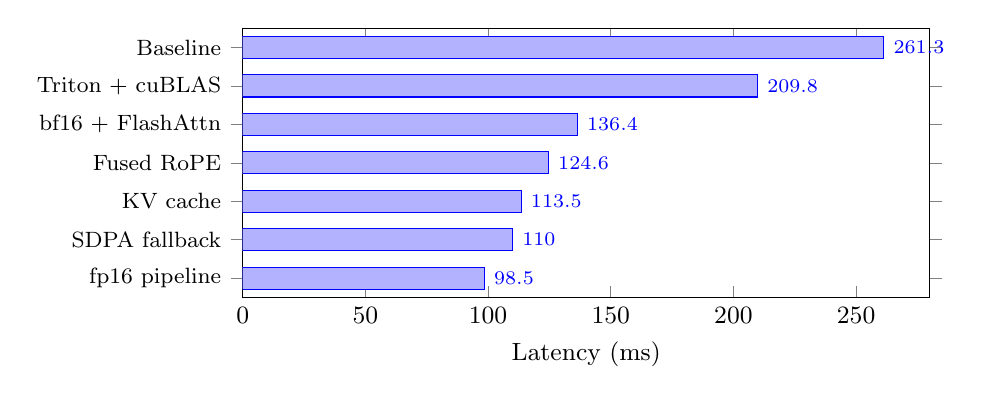
\begin{tikzpicture}
\begin{axis}[
    xbar,
    width=0.85\columnwidth,
    height=5.0cm,
    xlabel={Latency (ms)},
    xlabel style={font=\small},
    xmin=0, xmax=280,
    ytick={0,1,2,3,4,5,6},
    yticklabels={
      {Baseline},
      {Triton + cuBLAS},
      {bf16 + FlashAttn},
      {Fused RoPE},
      {KV cache},
      {SDPA fallback},
      {fp16 pipeline}
    },
    yticklabel style={font=\footnotesize},
    tick label style={font=\small},
    nodes near coords,
    nodes near coords style={font=\scriptsize, anchor=west},
    bar width=8pt,
    y dir=reverse,
    enlarge y limits={abs=0.5},
    every axis plot/.append style={fill=blue!60, draw=blue!80},
]
\addplot coordinates {
    (261.3, 0)
    (209.8, 1)
    (136.4, 2)
    (124.6, 3)
    (113.5, 4)
    (110.0, 5)
    (98.5, 6)
};
\end{axis}
\end{tikzpicture}
\vspace{-1ex}
\caption{Optimization progression (development GPU, RTX~5090).  Each bar shows end-to-end latency after applying all optimizations up to that step.  Optimizations validated on H200 at 204.8\,ms (Section~\ref{sec:comparison}).  Full breakdown in Appendix Table~\ref{tab:progression}.}
\label{fig:progression}
\end{figure}

\subsection{Tile/Block Size Tuning}

\textbf{Hypothesis:} Larger tiles amortize memory access overhead and improve compute utilization, but are constrained by shared memory capacity.

\textbf{Change:} We tested all valid tile configurations for the flash attention kernel---$(128,128)$, $(128,64)$, $(64,64)$, $(64,32)$, $(32,32)$, $(16,16)$---computing shared memory usage via Eq.~\ref{eq:smem} for each.  We also built an autotune system ($\sim$95 lines) that benchmarked each valid configuration at runtime.

\textbf{Result:} Initially, we used Triton's built-in \texttt{@triton.autotune} to select optimal tile configurations at runtime.  However, when tested, the autotune system selected $\texttt{BLOCK\_M}$=16 as optimal in micro-benchmarks, but the full-pipeline benchmark showed \textbf{101.6\,ms vs.\ 98.5\,ms} for our hand-tuned 64$\times$64 configuration---a 3.1\,ms regression.  We determined that the micro-benchmark methodology is too unreliable to capture full-pipeline cache effects.
In response, we developed a \texttt{GPUProfile} (\texttt{layers.py:89}) system with pre-tested configurations stored in \texttt{\_KNOWN\_CONFIGS} (\texttt{layers.py:23}). Unknown GPUs use dynamic computation largest-to-smallest against the shared memory budget.

We validated these choices through ablation testing on the H200 (Table~\ref{tab:ablation}), confirming that double-buffering and 8 warps are each worth $\sim$12\,ms, while fp16 contributes only +1.5\,ms on H200 (vs.\ $-$11.5\,ms on RTX~5090).

\begin{table}[h]
\centering
\caption{H200 ablation: top-impact parameter changes (baseline: 205.2\,ms).}
\label{tab:ablation}
\small
\begin{tabular}{@{}lrrl@{}}
\toprule
\textbf{Change} & \textbf{Time (ms)} & \textbf{$\Delta$} & \textbf{Insight} \\
\midrule
Disable fused RoPE & 234.1 & +28.9 & Most impactful fused kernel \\
\texttt{num\_stages}=1 & 217.4 & +12.2 & Double-buffering essential \\
\texttt{num\_warps}=4 & 217.2 & +12.0 & 128$\times$128 needs 8 warps \\
Decoder attn 32$\times$32 & 212.8 & +7.6 & Small tiles hurt \\
\texttt{num\_warps}=16 & 209.5 & +4.3 & Register pressure \\
SDPA fallback off & 208.6 & +3.4 & Custom kernel slow for seq\_q=1 \\
fp32 pipeline & 206.7 & +1.5 & Minimal on H200 (HBM3e) \\
Triton matmul & 206.2 & +1.0 & cuBLAS only slightly faster \\
MLP fusion off & 204.5 & $-$0.7 & Neutral (cuBLAS already fast) \\
\bottomrule
\end{tabular}
\end{table}

\latestsource{Source: \texttt{benchmarks/benchmarks\_ablation.md}; script: \texttt{hw1-asr/ablation\_test.py} via \texttt{hw1-asr/ablation\_job.sh}; generated artifacts: \texttt{hw1-asr/ablation\_results.\{json,md\}} and \texttt{hw1-asr/ablation\_output.log}.}

\subsection{Kernel Fusion}\label{sec:fusion}

\textbf{Hypothesis:} Fusing the SwiGLU pattern---$\text{SiLU}(\mathbf{x} \mathbf{W}_g) \odot (\mathbf{x} \mathbf{W}_u)$---into a single kernel eliminates two intermediate VRAM round-trips and three kernel launches per MLP layer.

\textbf{Change:} We wrote \texttt{swiglu\_fused\_kernel} (\texttt{layers.py:546}) that loads tiles of $\mathbf{x}$, $\mathbf{W}_g$, and $\mathbf{W}_u$ into shared memory, computes both matrix products in registers, applies SiLU and the element-wise multiply, and writes only the final result to VRAM.  The unfused path requires 5 kernel launches and 4 VRAM round-trips; the fused path requires 1 launch and 1 round-trip.

\textbf{Result:} With 28 decoder layers, fusion eliminates $\sim$84 kernel launches per inference.  For very small inputs (single-token decode, where $M < \texttt{TILE\_M}$), we fall back to cuBLAS, which has lower launch overhead for small matrices.
On the H200, MLP fusion contributes only $-$0.7\,ms (Table~\ref{tab:ablation}), because cuBLAS already saturates compute throughput for these matrix sizes.

\subsection{FlashAttention-Style Attention}

\textbf{Hypothesis:} The naive 3-kernel attention approach materializes the full $N_q \times N_k$ score matrix in VRAM, consuming $O(N_q \cdot N_k)$ memory and bandwidth.  A fused kernel with online softmax~\citep{milakov2018online} eliminates this materialization.

\textbf{Change:} We replaced the original 3-kernel pipeline (\texttt{attention\_scores}, \texttt{softmax\_inplace}, \texttt{attention\_output}) with a single \texttt{flash\_attention\_kernel} (\texttt{attention.py:34})~\citep{dao2023flashattention2fasterattentionbetter, ringlein2025anatomy}.  The kernel processes K/V in tiles of \texttt{BLOCK\_N} rows, maintaining running statistics $m_i$ (row-wise max) and $l_i$ (sum of exponentials) that are corrected as new tiles arrive.  The Q tile and accumulator $\mathbf{O}$ reside in registers; only the final output is written to VRAM.

Causal masking is handled via a compile-time \texttt{IS\_CAUSAL} flag that skips tiles entirely above the diagonal, avoiding wasted computation.  For single-token KV-cached decode (\texttt{seq\_q} $\leq$ 4), we fall back to PyTorch's \texttt{scaled\_dot\_product\_attention}, which has lower launch overhead for this degenerate case.

\textbf{Result:} \latestchglabel

\latestchgblock{\textbf{Latest update:} Section~5.3 now uses two clean submission-branch reruns, \texttt{2238637} and \texttt{2238638}, and \texttt{auto} is defined explicitly as the deployed mixed dispatch (flash for larger queries, SDPA fallback for tiny KV-cached decode steps), not as flash-only attention.}

\latestchgblock{We later reintroduced the original 3-kernel path behind \texttt{GLM\_ASR\_ATTENTION\_MODE=three\_kernel} and benchmarked it against the current deployed path.  Here, \texttt{auto} does \emph{not} mean ``flash everywhere'': it is the real deployed mixed dispatch, using the Triton flash kernel for larger \texttt{seq\_q} and PyTorch SDPA only for tiny KV-cached decode steps (\texttt{seq\_q}$\leq$4).  In two clean same-codebase reruns from the pushed submission branch, the student benchmark discards one full cold benchmark pass and averages three measured passes; under that methodology, the current path is consistently faster end-to-end (210.6--214.1\,ms vs.\ 280.8--291.9\,ms) while preserving 100\% accuracy.  The warmup-corrected detailed benchmark tells the same story: isolated component time falls from 823.49--826.69\,ms to 628.43--631.42\,ms ($\sim$1.3$\times$), with lower prefill (17.55--17.59$\rightarrow$12.96--13.15\,ms) and 50-step decode cost (742.55--745.70$\rightarrow$578.67--581.82\,ms).  These clean reruns therefore support FlashAttention-style dispatch as a substantial same-codebase improvement over the reintroduced materialized-score path.  The clean end-to-end justification for keeping the SDPA fallback remains Table~\ref{tab:ablation}: disabling it costs +3.4\,ms.}

\latestsource{Source: \texttt{benchmarks/benchmarks\_attention.md}; script: \texttt{hw1-asr/flash\_vs\_three\_kernel\_job.sh}; raw logs: \texttt{logs/h200\_attention\_2238637/} and \texttt{logs/h200\_attention\_2238638/}.}

\subsection{Other Optimizations}

\textbf{fp16-throughout pipeline.}
The original code called \texttt{.float()} after every Linear layer ($\sim$120 calls), doubling data size at each point.  Removing these conversions and keeping the entire pipeline in fp16 saves 11.5\,ms on the development GPU (RTX~5090).  On the H200, fp16 contributes only +1.5\,ms (Table~\ref{tab:ablation}), reflecting HBM3e's superior bandwidth.  Internal computation remains fp32 for numerical stability.

\textbf{KV-cache decoding (\texttt{generate\_v8b}).}
The stock \texttt{generate()} reprocesses the full growing sequence on every decode step ($O(n^2)$).  We implemented a KV-cached generation loop that processes only the new token each step, appending its K/V to a cache.  This is monkey-patched onto the model via \texttt{\_try\_patch\_v8b()} (\texttt{layers.py:1482}), called during \texttt{Linear.\_\_init\_\_}.  Impact on development GPU: $-$7.6\,ms.

\textbf{Fused Q+K RoPE kernel.}
RoPE requires applying the same rotation to both Q and K.  The baseline uses two separate kernel launches. We fuse them into \texttt{fused\_rope\_pair\_kernel} (\texttt{rope.py:189}), halving launch overhead.  On the H200, this is the most impactful single optimization: disabling it costs +28.9\,ms (Table~\ref{tab:ablation}). On the development GPU, impact was $-$11.8\,ms.


%======================================================================
\section{Comparison}\label{sec:comparison}
%======================================================================

\subsection{Data Collection}

We benchmark on the provided \texttt{test\_audio.wav} (3.5\,s, 16\,kHz, expected output: ``CONCORD RETURNED TO ITS PLACE AMIDST THE TENTS'').  Accuracy is measured by exact string match (case-insensitive) against the reference.  Each benchmark invocation runs 2 warmup + 5 timed iterations; we report 5 invocations (25 timed iterations total).  Both our implementation and the baseline are benchmarked under identical conditions.

\subsection{End-to-End Comparison}

\begin{table}[h]
\centering
\caption{End-to-end comparison on H200 MIG~3g.71gb (teaching cluster).}
\label{tab:comparison}
\small
\begin{tabular}{@{}lcccc@{}}
\toprule
\textbf{Implementation} & \textbf{Time (ms)} & \textbf{ms/tok} & \textbf{Accuracy} & \textbf{Speedup} \\
\midrule
Example baseline & 464.1 & 35.70 & 100\% & 1.00$\times$ \\
\textbf{Our template (fp16)} & \textbf{204.8} & \textbf{15.75} & \textbf{100\%} & \textbf{2.27$\times$} \\
\bottomrule
\end{tabular}
\end{table}

\latestsource{Source: \texttt{benchmarks/benchmarks.md}; script: \texttt{hw1-asr/benchmark\_student.py}; raw log: \texttt{logs/h200\_e2e\_2225992/benchmark\_raw\_output.txt}.}

\subsection{Per-Operator Comparison}

\chglabel\ \chg{Table~\ref{tab:peroperator} reports component-level timings on the H200 MIG~3g.71gb partition using \texttt{benchmark\_detailed.py} with one full warmup benchmark pass discarded and three measured benchmark passes averaged (each pass uses 5 timed runs per component).  These are isolated forward passes with 50 decode steps and \emph{no KV history}, so they measure steady-state operator latency rather than the algorithmic benefit of KV-cached generation.}

\begin{table}[h]
\centering
\caption{\chglabel\ \chg{Per-component comparison on H200 MIG~3g.71gb (isolated forward passes, 50 decode steps, 1 warmup benchmark discarded, average of 3 measured benchmark passes).}}
\label{tab:peroperator}
\small
\begin{tabular}{@{}lrrrr@{}}
\toprule
\textbf{Component} & \textbf{Ours (ms)} & \textbf{Baseline (ms)} & \textbf{Speedup} \\
\midrule
\chgcell{Audio Encoder} & \chgcell{36.53} & \chgcell{167.02} & \chgcell{4.57$\times$} \\
\chgcell{Projector} & \chgcell{0.14} & \chgcell{1.11} & \chgcell{7.93$\times$} \\
\chgcell{Decoder Prefill} & \chgcell{12.97} & \chgcell{20.51} & \chgcell{1.58$\times$} \\
\chgcell{Decoder Decode (50 steps)} & \chgcell{580.45} & \chgcell{817.09} & \chgcell{1.41$\times$} \\
\midrule
\chgcell{Total} & \chgcell{630.09} & \chgcell{1005.73} & \chgcell{1.60$\times$} \\
\bottomrule
\end{tabular}
\end{table}

\latestsource{Source: \texttt{benchmarks/benchmarks\_detailed.md}; script: \texttt{hw1-asr/benchmark\_detailed.py} via \texttt{hw1-asr/benchmark\_detailed\_job.sh}; raw logs: \texttt{logs/h200\_detailed\_2236079/}.}

\subsection{Root Cause Analysis}

All optimizations preserve full transcription accuracy: fp16 introduces no degradation because internal kernel computation remains in fp32, and KV-cached decoding produces identical token sequences to the stock path.

\chglabel\ \chg{In the steady-state H200 component profile, our implementation is faster in every stage.  The largest absolute saving comes from decoder decode (817.09\,ms $\to$ 580.45\,ms over 50 steps), while audio encoding and the projector also improve substantially once Triton compilation warmup is removed from the measurement.}

\chglabel\ \chg{The isolated component table understates the full end-to-end speedup because \texttt{benchmark\_detailed.py} does not use KV-cached generation.  Table~\ref{tab:comparison}, by contrast, uses the full student benchmark with \texttt{generate\_v8b}.  The end-to-end result therefore benefits from both faster steady-state kernels \emph{and} the algorithmic reduction from quadratic reprocessing to linear-time cached decode.  This explains why the per-component total speedup is 1.60$\times$ while the full H200 pipeline reaches 2.27$\times$.}

\chglabel\ \chg{\textbf{1. Faster steady-state kernels in both encoder and decoder.}
Flash attention, fused RoPE, fp16 norms, and fused MLP kernels reduce operator time throughout the pipeline.  On H200 this appears as 4.57$\times$ faster audio encoding, 1.58$\times$ faster decoder prefill, and 1.41$\times$ faster decode steps in isolated profiling.}

\chglabel\ \chg{\textbf{2. KV-cached generation in the end-to-end path.}
The detailed benchmark measures single-step decode without KV history, but the full inference benchmark uses our KV-cached \texttt{generate\_v8b}.  That cached path avoids recomputing attention over the full growing sequence at every token and therefore contributes additional end-to-end speedup beyond the isolated operator table.}

\textbf{Cross-GPU generalization.}
To verify portability, we evaluated on both the teaching cluster (H200 MIG) and a consumer GPU (RTX~5090).
The \texttt{GPUProfile} system correctly adapts tile sizes and pipeline stages to each architecture's shared memory budget.
Table~\ref{tab:crossgpu_main} confirms consistent speedups across both GPUs.

\begin{table}[h]
\centering
\caption{Cross-GPU comparison: teaching cluster vs.\ consumer GPU.}
\label{tab:crossgpu_main}
\small
\begin{tabular}{@{}lrrrrr@{}}
\toprule
\textbf{GPU} & \textbf{SMs} & \textbf{VRAM} & \textbf{Ours (ms)} & \textbf{Baseline (ms)} & \textbf{Speedup} \\
\midrule
H200 MIG 3g.71gb & 60 & 70\,GB & 204.8 & 464.1 & 2.27$\times$ \\
RTX~5090 (full) & 170 & 32\,GB & 100.4 & 262.2 & 2.61$\times$ \\
\bottomrule
\end{tabular}
\end{table}

\latestsource{Source: H200 row from \texttt{benchmarks/benchmarks.md} (\texttt{logs/h200\_e2e\_2225992/benchmark\_raw\_output.txt}); RTX~5090 row from \texttt{benchmarks/benchmarks\_5090.md} (embedded transcript from \texttt{hw1-asr/benchmark\_student.py}).}

\chglabel\ \chg{The RTX~5090 row in Table~\ref{tab:crossgpu_main} comes from a later confirmation rerun (100.4\,ms vs.\ 262.2\,ms), whereas Appendix Table~\ref{tab:progression} preserves the original development benchmark chain (261.3\,ms $\rightarrow$ 98.5\,ms).  We keep the full progression table on a single coherent benchmark session so that the per-step deltas remain meaningful.}

%======================================================================
\section{Conclusion}\label{sec:conclusion}
%======================================================================

\textbf{Most impactful optimization.}
On the H200, our optimizations reduced inference from 464.1\,ms to 204.8\,ms (2.27$\times$).
Ablation testing (Table~\ref{tab:ablation}) revealed that fused RoPE (+28.9\,ms when disabled), double-buffering (+12.2\,ms), and warp count (+12.0\,ms) collectively account for $>$53\,ms---kernel launch reduction and memory-latency hiding dominate over precision or tile-size changes on this architecture.

\textbf{Key lessons.}
(1)~The pipeline is overwhelmingly \emph{memory-bandwidth-bound}: halving data types (fp32$\to$fp16) and eliminating intermediate writes (kernel fusion, flash attention) provided the largest gains.
(2)~Attention is the most challenging kernel to optimize because tile size, shared memory, warp count, and pipeline stages are tightly coupled; the H200's 228\,KB shared memory accommodates 128$\times$128 tiles with double-buffering, while consumer GPUs with $\sim$99\,KB require 64$\times$64 with single-buffering---demonstrating the need for a portable \texttt{GPUProfile} system.
\chglabel\ \chg{(3)~Profile before optimizing: warmup-corrected component profiling confirms that decoder decode, not the compute-heavy linear projections, remains the dominant bottleneck---decode steps (bandwidth-bound attention + KV reads) still consume 92.1\% of the isolated component total on H200 even after optimization.}
(4)~Testing each kernel independently is straightforward; however, problems arise when kernels are composed in the full pipeline, as cache interactions between adjacent kernels produce behaviors not visible in isolated benchmarks.

\textbf{Surprising findings.}
Autotune found \emph{worse} configs than hand-tuning (micro-benchmarks miss cache effects). Encoder attention is compute-bound on H200 but bandwidth-bound on consumer GPUs---the same kernel has different bottlenecks across architectures.
\textbf{Future work:} \texttt{torch.compile}, speculative decoding, FP8 quantization, and per-architecture SDPA threshold tuning.

\clearpage
\bibliography{mybib}
\bibliographystyle{iclr2025_conference}

\appendix
\section{Appendix}

\subsection{Full Optimization Progression}

\chglabel\ \chg{Table~\ref{tab:progression} shows every optimization step from the original RTX~5090 development benchmark chain.  These step-by-step values are intentionally kept from one session (261.3\,ms baseline to 98.5\,ms final) rather than mixed with the later 100.4\,ms confirmation rerun used in Table~\ref{tab:crossgpu_main}.}

\begin{table}[h]
\centering
\caption{Complete optimization progression (RTX~5090, 3.5\,s audio, 13 tokens).}
\label{tab:progression}
\small
\begin{tabular}{@{}rlrrl@{}}
\toprule
\textbf{\#} & \textbf{Change} & \textbf{Time} & \textbf{$\Delta$} & \textbf{Mechanism} \\
\midrule
0 & Baseline & 261.3 & --- & fp32, 3-kernel attn, $O(n^2)$ \\
1 & Triton kernels + cuBLAS + TF32 & 209.8 & $-$51.5 & Custom kernels + tensor cores \\
2 & bf16 weights + Flash Attention & 136.4 & $-$73.4 & Half bandwidth + fused attn \\
3 & Fused Q+K RoPE pair kernel & 124.6 & $-$11.8 & Halved RoPE launches \\
4 & bf16 RMSNorm output & 120.7 & $-$3.9 & Eliminated type conversion \\
5 & bf16 LayerNorm output & 121.1 & $-$0.7 & Same for encoder norms \\
6 & KV cache (\texttt{generate\_v8b}) & 113.5 & $-$7.6 & $O(n) $ decoding \\
7 & SDPA fallback (seq\_q $\leq$ 4) & 110.0 & $-$3.5 & Lower overhead for decode \\
8 & fp16 cuBLAS HGEMM & 109.6 & $-$0.4 & fp16 slightly faster than bf16 \\
9 & Remove \texttt{.float()} casts & 102.1 & $-$7.5 & Eliminated $\sim$120 fp32 casts \\
10 & Remove activation fp32 casts & 98.4 & $-$3.7 & SiLU/GELU stay fp16 \\
11 & Remove norm fp32 casts & 98.1 & $-$0.3 & Norms output fp16 directly \\
12 & fp16 embeddings + fused MLP & \textbf{98.5} & $+$0.4 & Pipeline complete (noise) \\
\bottomrule
\end{tabular}
\end{table}

\latestsource{Source: \texttt{benchmarks/benchmarks\_history.md}; historical RTX~5090 development record extracted from pre-cleanup docs at branch base \texttt{f8c2f36}.}

\subsection{Rejected Optimizations}

\begin{table}[h]
\centering
\caption{Optimizations tested and rejected with measured results.}
\label{tab:rejected}
\small
\begin{tabular}{@{}lrl@{}}
\toprule
\textbf{Optimization} & \textbf{Impact} & \textbf{Reason for Rejection} \\
\midrule
Grid swizzling (SwiGLU) & +18\,ms & RTX~5090 L2 (98\,MB) already has good locality \\
\texttt{@triton.autotune} (GELU/SiLU) & +0.7\,ms & Tuning warmup exceeds possible gain \\
Flash Attn \texttt{num\_stages}=2 & Crash & RTX~5090 99\,KB cannot hold two tile buffers \\
SDPA for all attention & +6\,ms & Custom kernel faster for long sequences \\
SDPA \texttt{enable\_gqa} & +13\,ms & Manual KV expansion is faster \\
Warmup autotune & +3.1\,ms & Micro-benchmarks chose suboptimal configs \\
\bottomrule
\end{tabular}
\end{table}

\latestsource{Source: \texttt{benchmarks/benchmarks\_history.md}; historical RTX~5090 development record extracted from pre-cleanup docs at branch base \texttt{f8c2f36}.}

\subsection{Benchmark Source Map}
\label{app:benchmap}

\latestchgblock{This subsection provides a direct trace from the main benchmark-backed report claims to their canonical benchmark documents, scripts, and raw artifacts. The intended lookup path is: report table $\rightarrow$ canonical benchmark doc $\rightarrow$ script/runner $\rightarrow$ raw artifact or generated result file.}

{\footnotesize
\noindent\latestchglabel\ \textbf{Main benchmark source map.}

\medskip
\noindent\textbf{\texttt{tab:e2e}, \texttt{tab:comparison}.}
Canonical doc: \texttt{benchmarks.md}.
Script: \texttt{benchmark\_student.py}.
Artifact: H200 e2e bundle \texttt{h200\_e2e\_2225992}.

\medskip
\noindent\textbf{\texttt{tab:detailed}, \texttt{tab:peroperator}.}
Canonical doc: \texttt{benchmarks\_detailed.md}.
Script: \texttt{benchmark\_detailed.py} and \texttt{benchmark\_detailed\_job.sh}.
Artifact: H200 detailed bundle \texttt{h200\_detailed\_2236079}.

\medskip
\noindent\textbf{\texttt{tab:ablation}.}
Canonical doc: \texttt{benchmarks\_ablation.md}.
Script: \texttt{ablation\_test.py} and \texttt{ablation\_job.sh}.
Artifact: generated files \texttt{ablation\_results.json} and \texttt{ablation\_results.md}.

\medskip
\noindent\textbf{\texttt{tab:crossgpu\_main} (H200).}
Canonical doc: \texttt{benchmarks.md}.
Script: \texttt{benchmark\_student.py}.
Artifact: same H200 e2e bundle \texttt{h200\_e2e\_2225992}.

\medskip
\noindent\textbf{\texttt{tab:crossgpu\_main} (RTX~5090).}
Canonical doc: \texttt{benchmarks\_5090.md}.
Script: \texttt{benchmark\_student.py}.
Artifact: embedded confirmation transcript in the benchmark doc.

\medskip
\noindent\textbf{Section~5.3.}
Canonical doc: \texttt{benchmarks\_attention.md}.
Script: \texttt{flash\_vs\_three\_kernel\_job.sh}.
Artifact: H200 attention bundles \texttt{h200\_attention\_2238637} and \texttt{h200\_attention\_2238638}.

\medskip
\noindent\textbf{\texttt{tab:progression}, \texttt{tab:rejected}.}
Canonical doc: \texttt{benchmarks\_history.md}.
Script/runner: historical development runs.
Artifact: extracted history at branch base \texttt{f8c2f36}.
\par}

\subsection{Code Map}

\latestchglabel

\latestchgblock{Following the C4 model's idea of creating ``maps of your code'' through progressively higher-level abstractions, and arc42's level-1 building-block view, Table~\ref{tab:codemap} groups the supplementary code by building block, responsibility, and primary source location rather than listing every kernel symbol individually. This gives a grader a top-down navigation aid first; the benchmark source map above then provides the trace from report claims to benchmark scripts and artifacts.}

\begin{table}[h]
\centering
\caption{\latestchglabel\ Level-1 building-block map of the supplementary code.}
\label{tab:codemap}
\footnotesize
\begin{tabularx}{\linewidth}{@{}p{0.17\linewidth}YYp{0.15\linewidth}@{}}
\toprule
\textbf{Building block} & \textbf{Responsibility} & \textbf{Primary files / entry points} & \textbf{Report use} \\
\midrule
Benchmark harness & Runs the end-to-end, detailed, ablation, and attention-backend experiments; writes the logs that feed the benchmark documents. & \texttt{benchmark\_student.py}, \texttt{benchmark\_detailed.py}, \texttt{ablation\_test.py}, \texttt{flash\_vs\_three\_kernel\_job.sh} & Tables~\ref{tab:e2e}, \ref{tab:detailed}, \ref{tab:ablation}; Sec.~5.3 \\
Optimized template runtime & Selects GPU-specific tile and pipeline choices, wires the fused Triton kernels into the model, and implements KV-cached generation. & \texttt{template/layers.py} with \texttt{GPUProfile} and \texttt{generate\_v8b} as the main runtime entry points & Secs.~3--5, conclusion \\
Attention subsystem & Implements the deployed mixed attention dispatch: FlashAttention for long sequences, SDPA fallback for tiny decode steps, and the reintroduced 3-kernel path for controlled comparison. & \texttt{template/attention.py} with \texttt{flash\_attention\_kernel} and the mode-controlled attention wrapper & Sec.~5.3, Table~\ref{tab:peroperator} \\
RoPE subsystem & Applies rotary position embeddings with a fused kernel path and the runtime wrapper used by the decoder. & \texttt{template/rope.py} with \texttt{fused\_rope\_pair\_kernel} and \texttt{apply\_rotary\_pos\_emb} & Kernel fusion, appendix \\
Baseline reference implementation & Provides the comparison target for end-to-end and per-operator speedups against our optimized template. & \texttt{example/layers.py}, \texttt{example/attention.py}, and \texttt{example/rope.py} & Tables~\ref{tab:comparison}, \ref{tab:peroperator}, \ref{tab:crossgpu_main} \\
Evidence bundle & Stores the canonical benchmark writeups and the pulled raw H200 artifacts used to trace report numbers back to scripts and runs. & \texttt{benchmarks/*.md} and \texttt{logs/h200\_*} & Appendix A.2--A.3 \\
\bottomrule
\end{tabularx}
\end{table}

\latestsource{Structure based on two documentation patterns: the C4 model's abstraction-first code maps and arc42's level-1 building-block/source-mapping guidance. In practice, this table names a small set of coherent building blocks, states each block's responsibility, and points to the most important source locations rather than listing every kernel symbol.}

\end{document}
